\begin{pastexam}[label={px:ntu-106-esoe-ds-05}]{臺大工科海洋所 106 學年度 第 5 題}
（問答）

\textbf{(15 \%)} For the following graph as shown:
\begin{enumerate}[label=\alph*.]
\item (5 \%) Give the adjacency list representation.
\item (10 \%) Draw the minimum spanning tree.
\end{enumerate}

\begin{center}
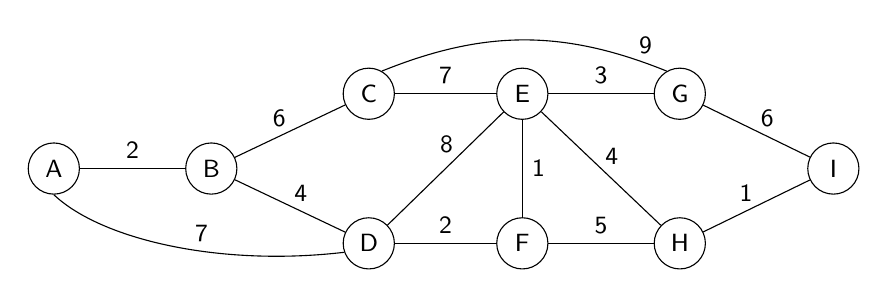
\begin{tikzpicture}[x=1.0cm,y=-1.0cm,
  v/.style={circle,draw,inner sep=0pt,minimum size=6.5mm,font=\sffamily\small},
  every node/.style={font=\sffamily\small}]
\node[v] (A) at (0.9,2.5) {A};
\node[v] (B) at (2.9,2.5) {B};
\node[v] (C) at (4.9,1.55) {C};
\node[v] (E) at (6.85,1.55) {E};
\node[v] (G) at (8.85,1.55) {G};
\node[v] (D) at (4.9,3.45) {D};
\node[v] (F) at (6.85,3.45) {F};
\node[v] (H) at (8.85,3.45) {H};
\node[v] (I) at (10.8,2.5) {I};
\draw (A) -- node[above] {2} (B);
\draw (B) -- node[above left=-2pt] {6} (C);
\draw (B) -- node[above right=-2pt] {4} (D);
\draw (A.south) .. controls (1.5,3.4) and (3.0,3.75) .. node[above,pos=0.6] {7} (D.200);
\draw (C) -- node[above] {7} (E);
\draw (E) -- node[above] {3} (G);
\draw (C.60) to[out=22,in=158] node[above,pos=0.93] {9} (G.120);
\draw (D) -- node[above left=-2pt,pos=0.6] {8} (E);
\draw (D) -- node[above] {2} (F);
\draw (E) -- node[right] {1} (F);
\draw (E) -- node[above right=-2pt] {4} (H);
\draw (F) -- node[above] {5} (H);
\draw (G) -- node[above right=-2pt] {6} (I);
\draw (H) -- node[above left=-2pt] {1} (I);
\end{tikzpicture}
\end{center}
\end{pastexam}

\begin{pastsoln}
答案：(a) 見下表；(b) 最小生成樹的邊是 E--F、H--I、A--B、D--F、E--G、B--D、E--H、B--C，總權重
$23$，而且這棵最小生成樹是唯一的。 (a) 屬資結書第~21~章，(b) 屬第~24~章，本題放在第~24~章。

\textbf{(a) 鄰接串列}（資結書第~21.2~節）。 無向圖的每條邊在兩端的串列各出現一次，$14$ 條邊
共 $28$ 個串列節點。 每個節點記「鄰點，權重」，串列裡的順序不影響正確性，這裡照字母排：
\begin{center}
\begin{tabular}{l@{\quad}l}
A & $\to$ (B, 2) $\to$ (D, 7) \\
B & $\to$ (A, 2) $\to$ (C, 6) $\to$ (D, 4) \\
C & $\to$ (B, 6) $\to$ (E, 7) $\to$ (G, 9) \\
D & $\to$ (A, 7) $\to$ (B, 4) $\to$ (E, 8) $\to$ (F, 2) \\
E & $\to$ (C, 7) $\to$ (D, 8) $\to$ (F, 1) $\to$ (G, 3) $\to$ (H, 4) \\
F & $\to$ (D, 2) $\to$ (E, 1) $\to$ (H, 5) \\
G & $\to$ (C, 9) $\to$ (E, 3) $\to$ (I, 6) \\
H & $\to$ (E, 4) $\to$ (F, 5) $\to$ (I, 1) \\
I & $\to$ (G, 6) $\to$ (H, 1) \\
\end{tabular}
\end{center}
每一列最後一個節點的 next 是 \NIL。 度數加起來 $2+3+3+4+5+3+3+3+2 = 28 = 2 \times 14$，
可以拿來檢查有沒有漏邊（資結書定理~21.1）。

\textbf{(b) 最小生成樹}，用 Kruskal 演算法（資結書第~24.2~節）：邊依權重由小到大看，兩端已經
在同一個集合就跳過，否則加入並合併。 權重相同的邊照字母順序看（結果不受影響，最後說明）。
\begin{center}
\small
\begin{tabular}{cclcl}
\toprule
權重 & 邊 & 結果 & 第幾條 & 加入後的集合（只列兩個點以上的） \\
\midrule
1 & E--F & 加入 & 1 & $\{E, F\}$ \\
1 & H--I & 加入 & 2 & $\{E, F\}$, $\{H, I\}$ \\
2 & A--B & 加入 & 3 & $\{A, B\}$, $\{E, F\}$, $\{H, I\}$ \\
2 & D--F & 加入 & 4 & $\{A, B\}$, $\{D, E, F\}$, $\{H, I\}$ \\
3 & E--G & 加入 & 5 & $\{A, B\}$, $\{D, E, F, G\}$, $\{H, I\}$ \\
4 & B--D & 加入 & 6 & $\{A, B, D, E, F, G\}$, $\{H, I\}$ \\
4 & E--H & 加入 & 7 & $\{A, B, D, E, F, G, H, I\}$ \\
5 & F--H & 跳過（同集合） & & \\
6 & B--C & 加入 & 8 & 全部 $9$ 個頂點 \\
\bottomrule
\end{tabular}
\end{center}
$9$ 個頂點的生成樹有 $8$ 條邊，到 B--C 就做完了，後面的 G--I (6)、A--D (7)、C--E (7)、D--E (8)、
C--G (9) 都不用看（它們的兩端都已經相連）。 總權重
$1 + 1 + 2 + 2 + 3 + 4 + 4 + 6 = 23$。 粗線是最小生成樹，虛線是沒選的邊：
\begin{center}
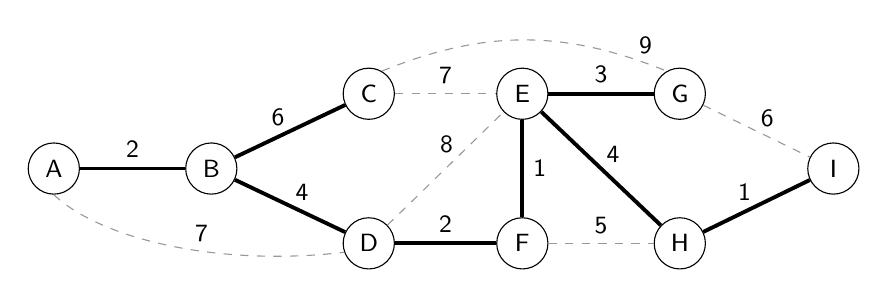
\begin{tikzpicture}[x=1.0cm,y=-1.0cm,
  v/.style={circle,draw,inner sep=0pt,minimum size=6.5mm,font=\sffamily\small},
  every node/.style={font=\sffamily\small},
  t/.style={line width=1.4pt}, n/.style={dashed,draw=black!40}]
\node[v] (A) at (0.9,2.5) {A};
\node[v] (B) at (2.9,2.5) {B};
\node[v] (C) at (4.9,1.55) {C};
\node[v] (E) at (6.85,1.55) {E};
\node[v] (G) at (8.85,1.55) {G};
\node[v] (D) at (4.9,3.45) {D};
\node[v] (F) at (6.85,3.45) {F};
\node[v] (H) at (8.85,3.45) {H};
\node[v] (I) at (10.8,2.5) {I};
\draw[t] (A) -- node[above] {2} (B);
\draw[t] (B) -- node[above left=-2pt] {6} (C);
\draw[t] (B) -- node[above right=-2pt] {4} (D);
\draw[n] (A.south) .. controls (1.5,3.4) and (3.0,3.75) .. node[above,pos=0.6] {7} (D.200);
\draw[n] (C) -- node[above] {7} (E);
\draw[t] (E) -- node[above] {3} (G);
\draw[n] (C.60) to[out=22,in=158] node[above,pos=0.93] {9} (G.120);
\draw[n] (D) -- node[above left=-2pt,pos=0.6] {8} (E);
\draw[t] (D) -- node[above] {2} (F);
\draw[t] (E) -- node[right] {1} (F);
\draw[t] (E) -- node[above right=-2pt] {4} (H);
\draw[n] (F) -- node[above] {5} (H);
\draw[n] (G) -- node[above right=-2pt] {6} (I);
\draw[t] (H) -- node[above left=-2pt] {1} (I);
\end{tikzpicture}
\end{center}

\textbf{唯一性。} 權重有重複，不能直接套「權重互異就唯一」。 改用環性質檢查：每條沒選的邊，
加進樹裡形成的環上，其他邊都比它\textbf{嚴格}小，它就不可能在任何最小生成樹裡（資結書
定理~24.3）。 F--H (5) 的環 F--E--H 上是 $1, 4$；G--I (6) 的環 G--E--H--I 上是 $3, 4, 1$；
A--D (7) 的環 A--B--D 上是 $2, 4$；C--E (7) 的環 C--B--D--F--E 上是 $6, 4, 2, 1$；D--E (8) 的
環 D--F--E 上是 $2, 1$；C--G (9) 的環 C--B--D--F--E--G 上是 $6, 4, 2, 1, 3$。 六條都成立，所以
最小生成樹只有這一棵，用 Prim 從哪個點開始也會得到同一棵。
\end{pastsoln}
